\chapter{Optimization: Problem Formulation and Solution}
\label{chap:batch}

Figure \ref{fig:batch_opti} gives an overview on how the batch optimization problem is solved.
On one hand, the real system is fed with some specific inputs and the system behaviour is measured by the available sensors.
On the other hand, virtual sensor measurements are calculated for the same inputs using a parameterized system model.
Our goal is to minimize the difference between the real and virtual system output.
\\

%For that, we formulate a cost function
%\begin{equation}
%S(\theta) = \sum_{j=1}^n ( y_j - f_j(x_j, \theta) )^2
%\end{equation}
%where $y_j$ are the measurements and $f_j(x_j, \theta)$ are the corresponding model outputs at time step $j$ and look for the parameters $\theta$ that minimize this function.
%\\

In the following, we will describe the system model and its parameters.
Then we show a solution to the problem as a nonlinear least squares formulation and derive an analytical solution for the parameter certainty.

\begin{figure}[btp]
\label{fig:batch_opti}
\centering
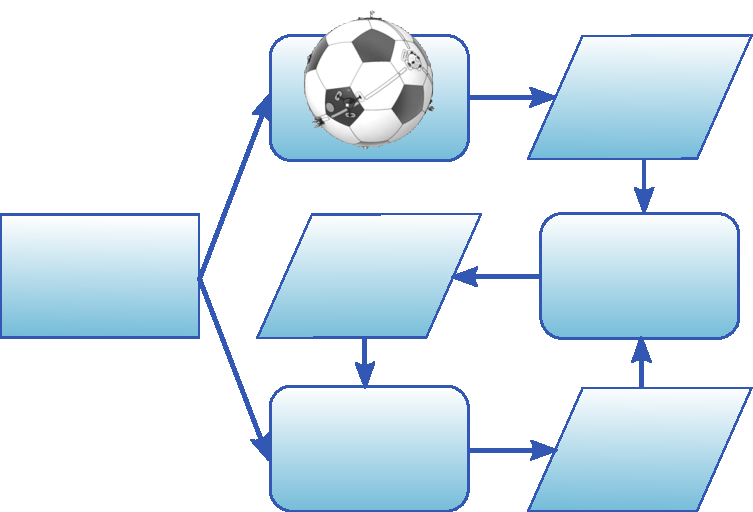
\includegraphics[width=0.85\textwidth]{images/problem_formulation.pdf}
\caption{Scheme for optimization of parameterized system model.}
\end{figure}

\section{System Model}
\label{sec:system_model}
A system model for Skye has been stated by \citet{Weichart2012} and is summarized in table \ref{tab:sys_mod}.

\begin{table}[htb!]
\centering
\label{tab:sys_mod}
$\begin{array}{ll}
\toprule
\dot{\boldsymbol{\omega}}_b^b &= \mathbf{J}_b^{-1} \left( \mathbf{M}_b  - \boldsymbol{\omega}_b^b \times \mathbf{J}_b \boldsymbol{\omega}_b^b \right) \\

\dot{\mathbf{q}}_w^{b,w} &= \frac{1}{2} \mathbf{q}_w^{b,w} \otimes \left[
\begin{array}{c}
	0 \\ \boldsymbol{\omega}_b^b
\end{array} \right] \\

\dot{\mathbf{v}}_b^b &= \mathbf{\mathcal{M}}_b^{-1} \mathbf{F}_b \\

\dot{\mathbf{p}}_w^{b,w} &= \mathbf{v}_w^b \\

\bottomrule
\end{array}$
\caption{Equations of motion for Skye}
\end{table}

It consists on the differential equations for the angular velocity $\boldsymbol{\omega}$, orientation quaternion $\mathbf{q}$, velocity $\mathbf{v}$, and position $\mathbf{p}$.
Skye is assumed as one rigid body.
Active forces and moments with respect to its center of gravity are concentrated as $\mathbf{F}$ and $\mathbf{M}$ respectively.
The total mass $\mathbf{\mathcal{M}}$ includes the rigid mass, helium mass as well as the virtual mass compensating for the inertia of the surrounding fluid.
The moment of inertia (or inertia tensor) $\mathbf{J}$ does not contain a virtual part as long as we focus on sphere like blimps.
\\
For the optimization, we content ourself with the angular acceleration $\boldsymbol{\alpha}$ as outlined in chapter \ref{chap:design_evaluation} and will have a closer look at the corresponding equation now.

\begin{equation}
\label{eq:angular_accel}
\boldsymbol{\alpha}_b^b = \mathbf{J}_b^{-1} \left( \mathbf{M}_b  - \boldsymbol{\omega}_b^b \times \mathbf{J}_b \boldsymbol{\omega}_b^b \right)
\end{equation}

The change of angular velocity is given by the active moments $\mathbf{M}$ as well as the nutation term $\boldsymbol{\omega} \times \mathbf{J} \boldsymbol{\omega}$.
\\
The latter term influences the rotation axis such that the free body will asymptotically end in a rotation around its smallest or or largest principle inertia axis.
For a homogeneous sphere, the inertia tensor is diagonal with all its diagonal elements equal and the cross product in \eqref{eq:angular_accel} is therefore zero (because $\boldsymbol{\omega}$ and $\mathbf{J}\boldsymbol{\omega}$ are parallel).
As Skye itself is not as perfect symmetric than a sphere (compare section \ref{sub:par_inertia}) the nutation term will be considered although it is much smaller than the active moment.
\\
As shown in \eqref{eq:moments}, the active moment consists of an actuation term $\mathbf{M}^{actuation}$, a gravitation term $\mathbf{M}^{gravity}$, and an aerodynamic term $\mathbf{M}^{aero}$.

\begin{equation}
\label{eq:moments}
\mathbf{M}_b = \underbrace{\sum_{k=1}^N  \left[  \mathbf{C}_{b,m_k} \left( \mathbf{p}^{m_k,cog}_{m_k} \times \mathbf{F}^k_{m_k} \right)  \right]}_{\mathbf{M}^{actuation}}
-
\underbrace{
 \left( \mathbf{p}^{cob,cog}_b \times (\mathbf{C}_{b,w}m\mathbf{g}_w) \right)
}_{\mathbf{M}^{gravity}}
+
\mathbf{M}^{aero}
\end{equation}

For the actuation term, the moment
(cross product between position vector $\mathbf{p}^{cog,m_k}$ from COG to thruster's point of action and motor force $\mathbf{F}^k$)
is first calculated in the local motor coordinate frames $m_k$ and then transformed by the rotation matrix $\mathbf{C}_{b,m_k}$ to blimp coordinates $b$ for each motor $k=1,...,N$.

The gravity term includes the offset $\mathbf{p}^{cob,cog}$ from COG to COB and 
the gravitation force $m\mathbf{g}$ which is transformed by the rotation matrix $\mathbf{C}_{b,w}$ from world coordinates $w$ to blimp coordinates $b$.

The aerodynamic term can be modelled as aerodynamic friction. According to \citet{Kundu2012}, the wall shear stress is usually expressed in terms of the dimensionless skin friction coefficient $c_f$ as 
\begin{equation*}
\tau_{wall} = 
\frac{1}{2} c_f \rho_{air} v^2 .
\end{equation*}

If only rotational movement of the blimp is considered, integrating the wall shear stress over the sphere leads to a moment counter acting the rotation with magnitude
\begin{align*}
\| \mathbf{M}^{aero} \|
&= \int_A \xi \tau_{wall} dA \\
&= \frac{1}{2} c_f \rho_{air} \int_A \xi (\xi \omega)^2 dA \\
&= \frac{1}{2} c_f \rho_{air} \omega^2 \int_{-r}^{r} (r^2-z^2)^{\frac{3}{2}} \sqrt{r^2-z^2} 2\pi dz \\
&= \frac{1}{2} c_f \rho_{air} \omega^2 \frac{32}{15} \pi r^5
\end{align*}

Nevertheless, this does not consider the drag of all components which are attached on the hull (e.g. actuation units or handles) which will have a large effect on the aerodynamics.
Measurements showed that the aerodynamic drag is more than a magnitude smaller than the usual actuation moments ($c_f \approx 0.02; \|\mathbf{M}^{aero}(\omega = \unit[0.8]{rad/s})\| \approx \unit[0.2]{Nm}$). Therefore we neglect this term and do not further bother about its direction.

%The position vector $\mathbf{p}^{m_k,cog}_{m_k}$ is expressed in motor coordinates too.
%As shown in section \ref{sub:par_position}, this simplifies the equation a lot if the motors are placed on a sphere. The motors forces $\mathbf{F}_{m_k}$ have only nonzero components in x and y direction (see figure \ref{fig:frames})
%
%\begin{equation}
%\mathbf{F}_{m_k} = \left[ \begin{array}{c}
%F_k\cos(\varphi_k) \\
%F_k\sin(\varphi_k) \\
%0
%\end{array} \right]
%\end{equation}
%
%and the thrust $F_k$ and angle $\varphi_k$ are accurately known for the selected data samples (compare section \ref{sub:data_selection}).

\section{Parameterization}
For the angular acceleration model introduced above, we formulate the parameterized system model as

\begin{eqnarray}
\label{eq:sys_mod}
\lefteqn{
\mathbf{f}(\mathbf{x}, \boldsymbol{\theta}) = {}} \\
& & {} \mathbf{J}_b^{-1} \left( 
\sum_{k=1}^N  \left[  \mathbf{C}_{b,m_k} \left( \mathbf{p}^{m_k,cog}_{m_k} \times \mathbf{F}^k_{m_k} \right)  \right]
-
\left( \mathbf{p}^{cob,cog}_b \times (\mathbf{C}_{b,w}m\mathbf{g}_w) \right)
- \boldsymbol{\omega}_b^b \times \mathbf{J}_b \boldsymbol{\omega}_b^b \right) \nonumber
\end{eqnarray}

Every variable in \eqref{eq:sys_mod} must either be a measurement, a known value or a parameter\footnote{In this work we only use time invariant variables.
As shown by \citet{Furgale2012}, continuous time variables can be added to batch optimization using spline functions.}. 
In our system model we can classify the variables as shown in table \ref{tab:params}.

\begin{table}[htb!]
\label{tab:params}
\centering
\begin{tabular}{lll}
\hline
Motor position & $\mathbf{p}^{m_k,cog}_{m_k}$ & param \\
Motor orientation & $\mathbf{C}_{b,m_k}$ & param \\
Blimp COG offset & $\mathbf{p}^{cob,cog}_b$ & param \\
Blimp inertia tensor & $\mathbf{J}_b$ & param \\
Blimp mass & $m$ & param \\
Input force & $\mathbf{F}_{m_k}^k$ & meas \\
Blimp orientation & $\mathbf{C}_{b,w}$ & meas \\
Blimp angular velocity & $\boldsymbol{\omega}$ & meas \\
Gravitation & $\mathbf{g}_w$ & known \\
\hline
\end{tabular}
\caption{Classification of all variables of the system model equation. All variables that are not known or measured, are introduced as a parameter.}
\end{table}

Since every additional parameter makes the problem harder to solve, we must focus on parameterizing \textit{hard to measure} values.
After an observability analysis in section \ref{sub:observability}, we will present an updated table where unobservable parameters are replaced by \textit{easy to measure} values.
%As we will show in section \ref{sub:observability}, a scale error in the 'knowns' $m$ and $\mathbf{g}$ result in a scale error of the COG offset estimate $\mathbf{p}^{cob,cog}$ only.
\\

There are several ways of how to represent the parameters.
We will show our choice in the sections below.

\subsection{Motor Position}
\label{sub:par_position}
In general, the motor position is a vector in the three dimensional space.
It points from the blimp's COG to the thruster's point of attack.
\begin{equation*}
\mathbf{p}^{m_k,cog}
=
\left[ \begin{array}{c}
p^{m_k,cog}_1 \\
p^{m_k,cog}_2 \\
p^{m_k,cog}_3
\end{array} \right]
\in \mathbb{R}^3
\end{equation*}
If we restrict the blimp hull to a perfect sphere, the ideal motor position vector space reduce to those vectors with length $r$.
The radius $r$ is the distance from the blimp's COG to the thruster's point of attack.
It is equal for all motors and the motor position expressed in the local motor frame $m_k$ (see figure \ref{fig:frames}) reduces to

\begin{equation}
\label{eq:motor_position}
\mathbf{p}^{m_k,cog}_{m_k}
=
\left[ \begin{array}{c}
0 \\
0 \\
-r
\end{array} \right]
\in \mathbb{R}^3
\end{equation}
The actual position on the hull is then simply given by the motor orientation, which is explained next.
The radius $r$ be measured by an appropriate measuring device.
As we will show in section \ref{sub:observability}, a scale offset of the now 'known' motor position leads to a scale offset of the estimates about the inertia tensor $\mathbf{J}$ and COG offset $\mathbf{p}^{cob,cog}$.

\subsection{Motor Orientation}
\label{sub:par_orientation}
Since the motor thrust is known in motor coordinates $m_k$, a transformation into blimp coordinates is necessary to calculate the dynamics of the blimp.
The coordinate transformation is described by a special orthogonal group in the three dimensional space (SO3).
The SO3 can either be minimal represented by $3$ parameters 
(e.g. Euler angles, rotation vector, Gibbs-Rodriquez parameters) 
or nonminimal represented by $p>3$ parameters and $p-3$ constraints 
(e.g. quaternions, rotation matrix).
While minimal representations always suffer from a singularity (there exists one specific rotation that is not described uniquely), nonminimal representations generally do not contain a singularity.
\\

Here we have to make the trade-off. Either we introduce one specific motor orientation which cannot be fully observed or we will have to solve a constraint optimization problem.
Unconstraint optimization problems are much less demanding to solve.
Therefore it is more convenient to choose a parameterization such that the motor orientation is not on the singularity.
If a rough estimate of the motor orientation can be made, this can be used to introduce an intermediate coordinate frame, such that the true motor orientation will not be on the singularity with very heigh probability.
Therefore, we go better with minimal representation for this problem\footnote{
An alternative implementation with nonminmal representation (quaternions) using either hard or soft constraints showed both worse performance than using minimal representation.
}.

Because of its computationally cheap and for optimization sufficiently smooth formula \eqref{eq:rod_to_C} to get the direction cosine transform, we use Gibbs-Rodriquez parameters $\boldsymbol{\lambda}$. Starting from rotation angle $\varphi$ and rotation axis $\mathbf{n}$, Gibbs-Rodriquez parameters are defined as

\begin{equation}
\boldsymbol{\lambda} = \mathbf{n} \tan(\varphi/2) 
\end{equation}

The direction cosine transform is calculated as

\begin{equation}
\label{eq:rod_to_C}
\mathbf{C} = \mathbf{I} + \frac{2}{1+\boldsymbol{\lambda}^\top \boldsymbol{\lambda}}
\left(\boldsymbol{\lambda}^\times + \left(\boldsymbol{\lambda}^\times\right)^2\right)
\end{equation}

\subsection{Inertia Tensor}
\label{sub:par_inertia}
The inertia tensor of a rigid body is calculated as
\begin{equation}
\mathbf{J} = \int_V \rho(x,y,z) 
\left[ \begin{array}{ccc}
y^2+z^2 & - xy    & - xz \\
- xy    & z^2+x^2 & - yz \\
- xz    & - yz    & x^2+y^2
\end{array} \right] dV
\end{equation}
and is always symmetric.
In its principle frame, the off-diagonal components are zero. We do not restrict the inertia tensor's principle frame to be aligned with the blimp frame $b$.
Therefore $\mathbf{J}_b$ is represented by six parameters.
\begin{equation}
\mathbf{J}_b = 
\left[ \begin{array}{ccc}
J_1 & J_4 & J_5 \\
J_4 & J_2 & J_6 \\
J_5 & J_6 & J_3
\end{array} \right]
\end{equation}


\subsection{Observability}
\label{sub:observability}
One way to analytically show observability of a system is shown by \citet{hermann1977} using Lie algebra. 
Here we do not show a proof of observability but rather argue qualitatively which parameters would not observable and are therefore not estimated.
As we find an optimal solution for the remaining parameters, we can assume that they are observable.
\\
For convenience, we state the parameterized system model \eqref{eq:sys_mod} again.

\begin{eqnarray*}
\lefteqn{
\mathbf{f}(\mathbf{x}, \boldsymbol{\theta}) = {}} \\
& & {} \mathbf{J}_b^{-1} \left( 
\sum_{k=1}^N  \left[  \mathbf{C}_{b,m_k} \left( \mathbf{p}^{m_k,cog}_{m_k} \times \mathbf{F}^k_{m_k} \right)  \right]
-
\left( \mathbf{p}^{cob,cog}_b \times (\mathbf{C}_{b,w}m\mathbf{g}_w) \right)
- \boldsymbol{\omega}_b^b \times \mathbf{J}_b \boldsymbol{\omega}_b^b \right)
\end{eqnarray*}

The first important observation is, that the scale of the inertia tensor $\mathbf{J}$ is only jointly observable with the scale of the position vectors of the motors $\mathbf{p}^{m_k,cog}$ and the COG offset $\mathbf{p}^{cob,cog}$.
If all those parameters have to be estimated, there exist infinite many solutions where the estimates are $\hat{\mathbf{p}}^{m_k,cog} = \gamma \mathbf{p}^{m_k,cog}$, 
$\hat{\mathbf{p}}^{cob,cog} = \gamma \mathbf{p}^{cob,cog}$ and 
$\hat{\mathbf{J}}           = \frac{1}{\gamma} \mathbf{J}$
for any real number $\gamma$.
The problem becomes observable, when the scale of one of those parameters is fixed, i.e. either the norm of one vector or the determinant of the tensor is assumed to be known.
Note that this scale can be chosen arbitrary with no impact on the motor orientation $\mathbf{C}_{b,m_k}$.

Because we simplified the motor position in \eqref{eq:motor_position} with the scalar radius $r$, it is sufficient to assume $r$ as known to get a unique solution for all remaining parameters.
Without this simplification, a constraint optimization problem has to be solved.
\\

If one has a look at the COG offset term in \eqref{eq:sys_mod}, it can be seen that the same scaling problem exists between $\mathbf{p}^{cob,cog}$ and $m$.
Here again, a wrong estimate of the fixed value $m$
\footnote{In contrast to the COG offset $\mathbf{C}_{b,m_k}$, the mass $m$ can easily be measured on scales. Therefore we assume the scalar $m$ as known.}
would only result in a scale error of the jointly observable parameter $\mathbf{p}^{cob,cog}$ without impact on the remaining parameters.
\\
For completeness, the updated classification of the variables from table \ref{tab:params} is shown in table \ref{tab:params_updated}.

\begin{table}[htb!]
\label{tab:params_updated}
\centering
\begin{tabular}{lll}
\hline
Motor orientation & $\mathbf{C}_{b,m_k}$ & param \\
Blimp COG offset & $\mathbf{p}^{cob,cog}_b$ & param \\
Blimp inertia tensor & $\mathbf{J}_b$ & param \\
Input force & $\mathbf{F}_{m_k}^k$ & meas \\
Blimp orientation & $\mathbf{C}_{b,w}$ & meas \\
Blimp angular velocity & $\boldsymbol{\omega}$ & meas \\
Gravitation & $\mathbf{g}_w$ & known \\
Blimp mass & $m$ & known \\
Motor POA radius & $r$ & known \\
\hline
\end{tabular}
\caption{dfdf}
\end{table}


\section{Nonlinear Least Squares}
As outlined above, our goal is to minimize the error between the measured and modelled angular acceleration.
For normally distributed system model errors, the maximum-likelihood estimate of the parameters \citep{Seber} is equivalent to find the solution to the least squares problem.
In general, the cost function $S(\boldsymbol{\theta})$ for the ordinary nonlinear least squares problem is

\begin{equation}
S(\boldsymbol{\theta}) = \sum_{i=1}^n ( y_i - f_i(\mathbf{x}_i, \boldsymbol{\theta}) )^2
\end{equation}
which is the squared sum of the residual between observation $y_i$ and function value $f_i(\mathbf{x}_i, \boldsymbol{\theta})$ for $n$ distinct observations.
For our problem, we group the observations to the three dimensional angular acceleration measurement vector $\mathbf{y}_j$ and the corresponding system model function $\mathbf{f}(\mathbf{x}_j, \boldsymbol{\theta})$ from \eqref{eq:sys_mod}

\begin{equation}
S(\boldsymbol{\theta}) = \sum_{j=1}^{n/3} \| \mathbf{y}_j - \mathbf{f}(\mathbf{x}_j, \boldsymbol{\theta}) \|^2
\end{equation}

and we have $n/3$ distinct angular acceleration measurements $\mathbf{y}_j$ at time step $j$.
For being consistent with the literature, we substitute the states $\mathbf{x}_j$ into the function $\mathbf{f}_j(\boldsymbol{\theta})$, and use from now on
\begin{equation}
\mathbf{f}(\boldsymbol{\theta}) = \left[ \begin{array}{c}
\mathbf{f}(\mathbf{x}_1, \boldsymbol{\theta}) \\
\vdots \\
\mathbf{f}(\mathbf{x}_{n/3}, \boldsymbol{\theta})
\end{array} \right]
, \qquad
\mathbf{y} = \left[ \begin{array}{c}
\mathbf{y}_1 \\
\vdots \\
\mathbf{y}_{n/3} 
\end{array} \right]
\end{equation}

and finally get the expression for the ordinary least squares problem

\begin{equation}
S(\boldsymbol{\theta}) = \| \mathbf{y} - \mathbf{f}(\boldsymbol{\theta}) \|^2
\end{equation}

The least squares solution to a linear problem 
$\mathbf{y} = \mathbf{X} \boldsymbol{\theta} + \boldsymbol{\varepsilon}$ 
with normally distributed error 
$\boldsymbol{\varepsilon} \sim \mathcal{N}(0,\mathbf{I} \sigma^2)$ 
can directly been calculated as (see \citep{Draper})

\begin{equation}
\boldsymbol{\theta} = (\mathbf{X}' \mathbf{X})^{-1} \mathbf{X}' \mathbf{y}
\end{equation}

where
\begin{equation}
\mathbf{V} (\boldsymbol{\theta}) = (\mathbf{X}' \mathbf{X})^{-1} {\sigma}^2
\end{equation}

is the covariance matrix of the estimates. An estimate for ${\sigma}$ is given by
\begin{equation}
\hat{\sigma}^2 = \frac{1}{n-p} (\mathbf{y} - \mathbf{X} \boldsymbol{\theta})
\end{equation}

To find a solution for nonlinear regression, iterative schemes have to be applied \citep{Seber}.
Linear Taylor expansion of the nonlinear function
$\mathbf{f}(\boldsymbol{\theta})$ 
for 
$\boldsymbol{\theta}$
close to 
$\boldsymbol{\theta}_0$
gives
\begin{equation}
\mathbf{f}(\boldsymbol{\theta}) \approx
\mathbf{f}(\boldsymbol{\theta}_0) + \mathbf{F}_0(\boldsymbol{\theta} - \boldsymbol{\theta}_0)
\end{equation}


%... Formulate minimization problem (unconstraint) as least-squares.
%... Cite \cite{Seber} (Nonlinear Regression) and maybe also \cite{Draper} (Applied Regression Analysis)

\section{Levenberg-Marquardt Algorithm}
... Again cite \cite{Seber} or directly Levenberg or Marquardt

\section{Jacobians / Derivatives}
... show how equations can be differentiated (for later use in LMA)

\section{Confidence Region}
... of parameters
... error propagation \cite{Siegwart}
